\chapter{評価実験}
\thispagestyle{fancy}


\section{評価方法}
図\ref{kankyou}のようにプロジェクターとKinectを配置する.
体験者はKinectの正面に立つ.
本研究で提案したプロジェクションマッピングをX人に体験してもらい,
評価を得るためにアンケートを実施した.

\vspace{1cm}
\begin{figure}[h]
  \centering
  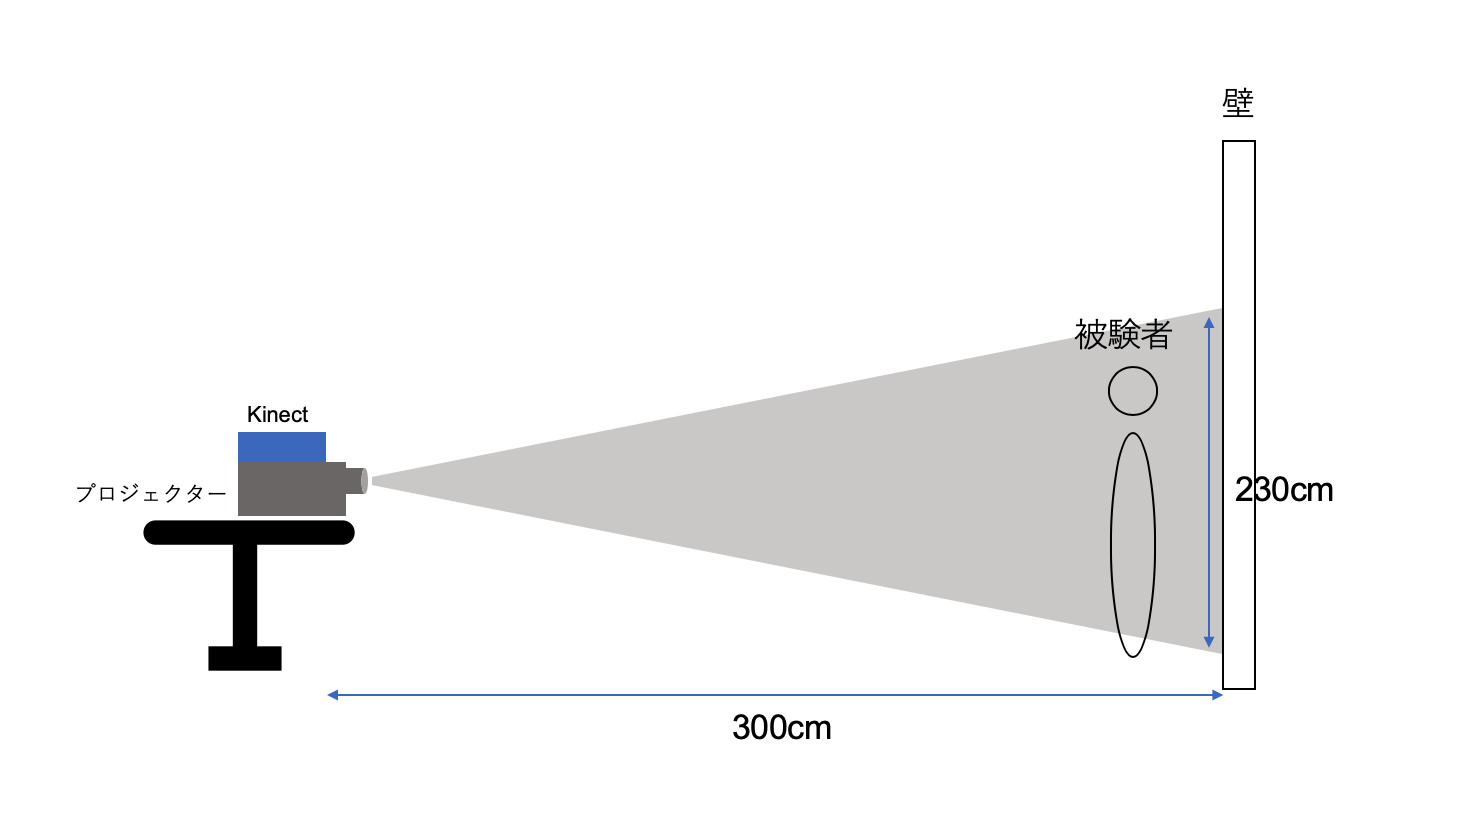
\includegraphics[width=14cm]{image/jikkenkankyou.png}
  \caption[実験環境図]{実験環境図.}
\label{kankyou}
\end{figure}


\clearpage

アンケートの質問内容を以下に示す.
\begin{itemize}
  \item[Q1.] 操作はわかりやすいか? [5段階評価]
  \item[Q2.] わかりづらかった場合,どこがわかりづらいか? 
  \item[Q3.] 楽しさについての満足感はどれくらいか? [5段階評価]
  \item[Q4.] 今後の改善点や意見・要望   
\end{itemize}



\section{評価結果}

